% !TeX root = ../praktikum.tex
% !TeX encoding = UTF-8
% !Tex spellcheck = de_DE

Wie zu den Messdaten der Gleich- und Wechselstrommessungen wurden die Ladungsträgerdichten und -beweglichkeiten hier für alle verschiedenen aufgenommenen Temperaturwerte von \unit[2]{K} bis \unit[40]{K} bestimmt. In der Abbildung~\ref{fig:temp_mess} ist der Längs-Spannungsverlauf zu verschiedenen Temperaturen abgebildet. Hierbei ist deutlich zu erkennen, wie die SDHO mit steigender Temperatur weniger stark ausgeprägt sind. Die Temperatur, ab welcher der Effekt nicht mehr zu erkennen ist, liegt zwischen $20$ und \unit[40]{K}.

Ladungsträgerdichte und -beweglichkeit wurden wie in den obigen Versuchsteilen über die Hall-Spannung berechnet und die Ergebnisse zu den verschiedenen Temperaturen in Tabelle~\ref{tab:temp_ausw} eingetragen.

\begin{table}[h]
	\centering
	\begin{tabular}{|l|r|l|r|r|}
		\hline
		\multicolumn{1}{|l|}{\cellcolor{black!30} $T$ } & \multicolumn{1}{|l|}{\cellcolor{black!30} $b$ } & \multicolumn{1}{|l|}{\cellcolor{black!30} $U_{xx}(B=0)$ } & \multicolumn{1}{|l|}{\cellcolor{black!30} $n_s$ } & \multicolumn{1}{|l|}{\cellcolor{black!30} $\mu$ } \\
		\multicolumn{1}{|l|}{\cellcolor{black!30} [$\unit{K}$] } &  \multicolumn{1}{|l|}{\cellcolor{black!30} [\unit{T}] } &
		\multicolumn{1}{|l|}{\cellcolor{black!30} [$\unit{V}$] } &  \multicolumn{1}{|l|}{\cellcolor{black!30} [$\unitfrac{1}{m^2}$] } & \multicolumn{1}{|l|}{\cellcolor{black!30} [$\unitfrac{m^2}{Vs}$] } \\ \hline
		$ 2 $  & $ 8,51422\cdot 10^{-4} $  & $ 2,73230\cdot 10^{-4} $  & $ 7,17948\cdot 10^{15} $  & $ 18,6968 $  \\ 
		$ 5 $  & $ 8,64040\cdot 10^{-4} $  & $ 2,84912\cdot 10^{-4} $  & $ 7,07464\cdot 10^{15} $  & $ 18,1959 $  \\ 
		$ 10 $  & $ 8,47763\cdot 10^{-4} $  & $ 2,80024\cdot 10^{-4} $  & $ 7,21046\cdot 10^{15} $  & $ 18,1648 $  \\ 
		$ 20 $  & $ 8,54649\cdot 10^{-4} $  & $ 2,99456\cdot 10^{-4} $  & $ 7,15237\cdot 10^{15} $  & $ 17,1240 $  \\ 
		$ 40 $  & $ 8,66678\cdot 10^{-4} $  & $ 3,48808\cdot 10^{-4} $  & $ 7,05310\cdot 10^{15} $  & $ 14,9081 $  \\ \hline
	\end{tabular}
	\caption{Berechnete Elektronendichte $n_s$ und -beweglichkeit $\mu$ in Abhängigkeit zu der Probentemperatur, aus Platzgründen ohne Fehler.}
	\label{tab:temp_ausw}
\end{table}


Die gleichen Ergebnisse sind zusätzlich in Abbildung~\ref{fig:temp_ausw} dargestellt. Um die Verläufe besser im Verhältnis zu verstehen, wurde die y-Achsenabschnitte in einem Bereich von $\pm \unit{15}[\%] $ um den Mittelwert gewählt. So sieht man, dass die Elektronendichte nahezu konstant verläuft, wohingegen ein leicht abnehmende Elektronenbeweglichkeit zu beobachten ist. Für die Elektronendichte ist keine einfache Abhängigkeit von der Temperatur bekannt, wohingegen die Elektronenbeweglichkeit durch die ansteigende Wechselwirkung abnehmen sollte. Beides spiegeln die Messergebnisse wider.

\begin{figure}[h]
	\centering
	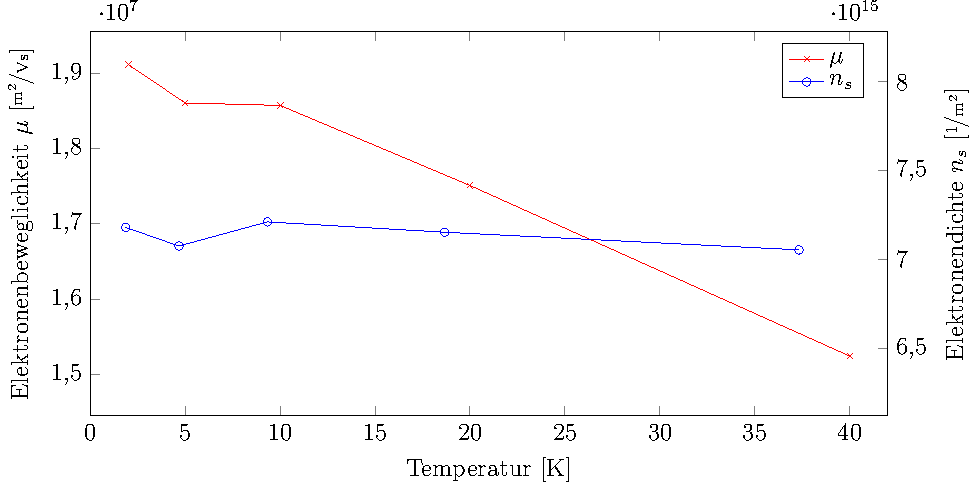
\includegraphics[scale=1]{graphs/temperatur/auswertung.pdf}
	\caption[Auswertung der Temperaturvariation]{
		Berechnete Elektronendichte $n_s$ und -beweglichkeit $\mu$ in Abhängigkeit zu der Probentemperatur. Fehlerbalken sind nicht eingetragen, da sie um mindestens eine Größenordnung kleiner sind als die Messergebnisse. Die Linien sind zur visuellen Führung eingezeichnet.
	}
	\label{fig:temp_ausw}
\end{figure}

